\documentclass[conference]{IEEEtran}
\IEEEoverridecommandlockouts
\usepackage{cite}
\usepackage{amsmath,amssymb}
\usepackage{graphicx}
\usepackage{booktabs}
\usepackage{multirow}
\usepackage{xcolor}
\usepackage{url}
\usepackage[hidelinks]{hyperref}

\newcommand{\fpb}{FPB}
\newcommand{\fiqa}{FiQA-SA}
\newcommand{\tfns}{TFNS}

\begin{document}

\title{Where to Spend the Parameters? Parameter-Efficient Domain Adaptation of Mixture-of-Experts Language Models for Financial NLP}

\author{\IEEEauthorblockN{Petr Tyukhmenev}
\IEEEauthorblockA{Deep Learning course project}}

\maketitle

\begin{abstract}
Sparse Mixture-of-Experts (MoE) language models store most of their parameters in experts
that are used conditionally, which raises a question that dense models do not have: when a
model is adapted to a new domain, where should the trainable parameters go? We study this for
financial text classification with Granite-3.1-1B-A400M, a 1.3B-parameter MoE model with 32
experts per layer, trained jointly on four sentiment and news-headline tasks. We compare LoRA
in the attention, budget-matched LoRA in the experts, tuning only the router, and
Expert-Specialized Fine-Tuning (ESFT), which updates the experts the model already uses most
on the target data, together with a random-expert control and ESFT-Specific, a variant that
selects the experts most specific to financial compared with general text. Over three seeds,
ESFT reaches 79.3\% mean macro-F1 (zero-shot: 42.0\%), the best and the most stable result,
on par with LoRA on a dense model of similar active size. Spending the same parameter budget
in the experts instead of the attention loses 8 points, and tuning the router alone falls
below zero-shot. ESFT-Specific is worse than random selection; a routing analysis shows why:
performance follows the share of routed tokens that pass through the tuned experts
(23\% for ESFT, 11\% random, 9\% domain-specific), not the specialisation of the experts.
Code, fixed splits, configurations and per-run results are available at
\url{https://github.com/2Gpb/Moe}.

\end{abstract}

\begin{IEEEkeywords}
mixture of experts, parameter-efficient fine-tuning, LoRA, domain adaptation, financial sentiment analysis
\end{IEEEkeywords}

\section{Introduction}

Sparse Mixture-of-Experts (MoE) transformers replace the dense feed-forward block with a set
of experts and a learned router that sends every token to a few of them~\cite{shazeer2017moe,fedus2022switch}.
The design decouples the number of stored parameters from the compute spent per token and is
now used in many open models~\cite{jiang2024mixtral,dai2024deepseekmoe,muennighoff2024olmoe,granite2024}.
Adapting such models to a specialised domain raises a question that does not exist for dense
networks: the parameters live in structurally different places (shared attention, many
conditionally used experts, and a small router that decides which experts are used), and a
limited budget of trainable parameters can be placed in any of them.

Standard parameter-efficient fine-tuning (PEFT) methods such as LoRA~\cite{hu2022lora} were
designed for dense models and are typically attached to the attention projections. For MoE
models, Wang et al.~\cite{wang2024esft} proposed Expert-Specialized Fine-Tuning (ESFT): routing
statistics on the target data identify the experts that the task already relies on, and only
those experts are updated. Whether this transfers to a small MoE model and to a domain shift
(rather than a task shift), and how it compares with LoRA in the attention or in the experts
and with a re-trained router, is the subject of this project.

We use financial text classification as the target domain. Financial sentiment differs from
everyday sentiment in a way that is easy to measure: a statement such as \emph{``the company
will publish its interim report on 5 May''} is neutral for an investor, and \emph{``operating
loss narrowed''} is positive although it contains the word ``loss''. A 1.3B-parameter MoE model
that reaches 93\% on the general-domain SST-2 benchmark scores only 33--37\% macro-F1 on two
financial sentiment datasets in our zero-shot evaluation, which makes the domain gap concrete.

\textbf{Contributions.}
\begin{itemize}
  \item A controlled comparison of four places for trainable parameters in a sparse MoE
  language model (attention LoRA, budget-matched expert LoRA, the router alone, and ESFT) on
  four financial classification tasks trained jointly, over three seeds, with a dense model of
  similar active size as reference.
  \item Two selection variants with the same expert budget as ESFT: random experts (control)
  and ESFT-Specific, our variant that ranks experts by how much more often they are used on
  financial than on general text.
  \item A routing analysis explaining the results: what matters for ESFT is the share of the
  routed computation that passes through the tuned experts, not how domain-specific they are,
  and tuning the router alone moves routing far more than the domain shift itself does.
  \item A compact, model-agnostic implementation of expert LoRA and expert deltas on top of the
  3D expert tensors used by current Hugging Face MoE models, released with fixed data splits
  and configurations.
\end{itemize}

\section{Related Work}

\textbf{Sparse Mixture-of-Experts.} The sparsely-gated MoE layer~\cite{shazeer2017moe} routes
each token to the top-$k$ of $E$ experts using a learned linear router. GShard and Switch
Transformer~\cite{lepikhin2021gshard,fedus2022switch} scaled the idea and introduced an
auxiliary load-balancing loss that keeps the experts uniformly used; ST-MoE~\cite{zoph2022stmoe}
studied fine-tuning stability and found that sparse models overfit more easily on small
downstream tasks. Recent open models use fine-grained experts (many small experts with a larger
$k$): DeepSeekMoE~\cite{dai2024deepseekmoe}, OLMoE~\cite{muennighoff2024olmoe} and IBM
Granite-MoE~\cite{granite2024}, which we use here. OLMoE reports domain-dependent routing,
which is the property ESFT and our analysis build on.

\textbf{Parameter-efficient fine-tuning.} Adapters~\cite{houlsby2019adapters} and
LoRA~\cite{hu2022lora} update a small number of new parameters while the backbone stays frozen;
QLoRA~\cite{dettmers2023qlora} combines LoRA with a quantised backbone. For MoE models,
ESFT~\cite{wang2024esft} fine-tunes only the experts that are most relevant to the downstream
data, measured either by the average gate score (ESFT-Gate) or by the fraction of tokens routed
to an expert (ESFT-Token). ESFT was evaluated on a 16B-parameter model and on task-specific
data (math, code, intent recognition, summarisation, legal judgement prediction and translation); we test it on a small model, on a domain rather than a
single task, and against budget-matched LoRA variants and selection controls.

\textbf{Financial NLP.} Financial sentiment benchmarks include Financial PhraseBank~\cite{malo2014fpb},
FiQA~\cite{maia2018fiqa}, gold-news headlines~\cite{sinha2021headlines} and Twitter financial
news~\cite{tfns2022}. Domain-specific models range from FinBERT~\cite{araci2019finbert}, an
encoder with continued pre-training, to BloombergGPT~\cite{wu2023bloomberggpt}, a 50B
decoder trained on a mixed financial and general corpus, and open instruction-tuned models
evaluated on FLARE/FinBen~\cite{xie2023pixiu,xie2024finben,yang2023fingpt}. Continued
pre-training is known to help domain transfer~\cite{gururangan2020dont} but is expensive; this
project studies the cheaper alternative of supervised parameter-efficient adaptation.

\section{Method}

\subsection{Sparse MoE block}
In every layer $\ell$ of the model the feed-forward block is replaced by $E$ experts. For a token
representation $x\in\mathbb{R}^{d}$ the router computes logits $r = W_r x$, $W_r\in\mathbb{R}^{E\times d}$,
keeps the top-$k$ experts $\mathcal{T}(x)$ and renormalises their scores:
\begin{equation}
  y = \sum_{e\in\mathcal{T}(x)} g_e(x)\, f_e(x),\quad
  g_e(x) = \frac{\exp r_e}{\sum_{j\in\mathcal{T}(x)} \exp r_j},
\end{equation}
where each expert is a gated MLP $f_e(x) = D_e\,[\,\mathrm{SiLU}(G_e x)\odot U_e x\,]$ with
$G_e,U_e\in\mathbb{R}^{m\times d}$ and $D_e\in\mathbb{R}^{d\times m}$. In current Hugging Face
implementations all experts of a layer are stored in two tensors,
$[G;U]\in\mathbb{R}^{E\times 2m\times d}$ and $D\in\mathbb{R}^{E\times d\times m}$, so expert
parameters are not \texttt{nn.Linear} modules and off-the-shelf LoRA libraries cannot target
them directly.

\subsection{Classification with the language-model head}
All tasks are cast as next-token prediction. An instruction, the input text and the cue
\texttt{Answer:} form the prompt; each class $c$ is mapped to one verbalizer token
$v_c$ (\texttt{negative}/\texttt{neutral}/\texttt{positive} or \texttt{No}/\texttt{Yes})~\cite{schick2021pet}.
With $h$ the final hidden state at the last prompt position and $W_o$ the output embedding,
\begin{equation}
  p(c\mid \text{prompt}) = \operatorname{softmax}_{c}\big( W_o[v_c]^{\top} h \big),
\end{equation}
and training minimises the cross-entropy of this restricted distribution. The same scoring is
used for zero-shot, few-shot and fine-tuned models, so differences come only from the
parameters. Only the last position is projected onto the vocabulary, which avoids
materialising a $B\times L\times|V|$ logit tensor.

\subsection{Where to place the trainable parameters}
All methods keep the pre-trained weights frozen and differ only in which tensors are trained.

\textbf{Attention LoRA.} Each of $W_q,W_k,W_v,W_o$ becomes $W + \frac{\alpha}{r}BA$ with
$A\in\mathbb{R}^{r\times d_\text{in}}$, $B\in\mathbb{R}^{d_\text{out}\times r}$, $B=0$ at initialisation~\cite{hu2022lora}.

\textbf{Expert LoRA.} Every expert receives its own low-rank update on both projections,
$[G;U]_e + \frac{\alpha}{r}B^{gu}_e A^{gu}_e$ and $D_e + \frac{\alpha}{r}B^{d}_e A^{d}_e$.
The adapters are stored as 3D tensors aligned with the expert dimension. With rank $r=1$ the
number of trainable parameters (2.75M) matches attention LoRA with $r=16$, which gives a
budget-matched comparison of \emph{attention vs.\ experts}.

\textbf{Router tuning.} Only $W_r$ of every layer is trained (0.79M parameters). Changing the
router does not change what an expert computes, only which experts are used and with what
weight, so this tests whether re-routing alone can adapt the model to the domain.

\textbf{ESFT.} Following~\cite{wang2024esft}, we run the frozen model over the financial
training data and compute, for every layer and expert, the token selection ratio
$s_{\ell,e} = \frac{1}{kN}\sum_{t} \mathbb{1}[e\in\mathcal{T}(x_t)]$ (ESFT-Token).
In each layer the smallest set of experts whose cumulative score reaches $p=0.2$ is selected,
and only those experts are updated with full-rank deltas $\Delta_e$ initialised at zero. For
Granite this selects 82 of the 768 experts (2--4 per layer), i.e.\ 129M trainable parameters.
Padding positions are excluded from the statistics. The deltas are kept in fp32 and applied as
a separate product $x\Delta_e^\top$; adding them to a half-precision weight first would round
small updates away.

\textbf{ESFT-Specific.} The experts with the highest usage on financial data are mostly used
just as heavily on any text (Fig.~\ref{fig:spec}). We therefore also rank experts by domain
specificity, the log-ratio of their selection ratio on financial and general-domain text,
\begin{equation}
  \sigma_{\ell,e} = \log \frac{s_{\ell,e}(\text{fin})}{s_{\ell,e}(\text{general})},
\end{equation}
and select, in every layer, the same number of experts as ESFT-Token but with the largest
$\sigma$. General-domain statistics come from SST-2~\cite{socher2013sst} sentences, i.e.\ the
same task (sentiment) in a different domain, so $\sigma$ isolates the domain rather than the task.

\textbf{Control.} To test whether the \emph{choice} of experts matters at all, ESFT-Random
updates the same number of experts per layer, chosen uniformly at random (a different draw for
every seed).

\subsection{Implementation}
The adapted experts module sorts the $kN$ (token, expert) pairs by expert, lets every expert
process its contiguous slice, and scatters the weighted outputs back. This is the grouped-GEMM
pattern written as a plain loop, so the same code runs on CUDA, Apple MPS and CPU and works for
any model with the router/experts layout above (Granite-MoE, OLMoE, Qwen-MoE, Mixtral).
Without adapters the module reproduces the original forward pass to $10^{-5}$, which is
checked by unit tests together with gradient flow and parameter counts.

\section{Experimental Setup}

\subsection{Data}
Table~\ref{tab:data} lists the tasks. \fpb{}, \fiqa{} and Headlines use the FLARE
splits~\cite{xie2023pixiu}. \tfns{} has no public test set; its official validation split is
our test set and a stratified 10\% of the training data is held out for validation. Headlines
asks several yes/no questions about the same headline (price up/down, past/future news, \ldots);
we remove from training every headline that appears in validation or test, so that no headline
is seen under a different question. The two large sources are subsampled with a fixed seed
(Table~\ref{tab:data}); all splits are stored as files in the repository.
SST-2~\cite{socher2013sst} (872 validation sentences) is used only as the general-domain
reference for the routing analysis and is never trained on.

\begin{table}[t]
\centering
\caption{Tasks and split sizes after subsampling.}
\label{tab:data}
\begin{tabular}{l l c r r r}
\toprule
Task & Source & Cls. & Train & Val & Test \\
\midrule
\fpb{} & news sentences~\cite{malo2014fpb} & 3 & 3100 & 776 & 970 \\
\fiqa{} & posts, microblogs~\cite{maia2018fiqa} & 3 & 750 & 188 & 235 \\
\tfns{} & tweets~\cite{tfns2022} & 3 & 2500 & 500 & 2388 \\
Headlines & gold news~\cite{sinha2021headlines} & 2 & 2500 & 500 & 2000 \\
SST-2 & movie reviews~\cite{socher2013sst} & 2 & -- & -- & 872 \\
\bottomrule
\end{tabular}
\end{table}

\subsection{Models}
The main model is Granite-3.1-1B-A400M-base~\cite{granite2024}: 24 layers, hidden size 1024,
32 experts per layer with intermediate size 512, top-8 routing, 1.33B parameters in total and
about 0.4B active per token. As a dense reference we use Qwen2.5-0.5B~\cite{qwen2025qwen25}
(0.49B parameters, all active) with the same attention LoRA.

\subsection{Training}
One adapter is trained on the union of the four training sets for one epoch (553 steps of
batch size 16) with AdamW~\cite{loshchilov2019adamw}, no weight decay, 6\% linear warm-up and
cosine decay, gradient clipping at 1.0 and maximum prompt length 192 tokens (longer prompts are
truncated from the left so that the answer cue is kept). The learning rate
is $2\cdot10^{-4}$ for LoRA, $5\cdot10^{-4}$ for the router and $3\cdot10^{-5}$ for the
full-rank ESFT deltas; LoRA uses $\alpha=2r$. The frozen backbone runs in fp16 with dynamic
loss scaling and all trainable tensors are kept in fp32. The validation set is evaluated every 200 steps and at
the end, and the adapter with the best mean validation macro-F1 is used for testing. No
hyper-parameter search was performed: the values follow common practice for each method and
are identical across tasks. Every configuration is trained with three seeds (0, 1, 2), which
change the data order, the LoRA initialisation and, for ESFT-Random, the chosen experts. All
runs use a single NVIDIA T4 (16\,GB) on Kaggle.

\textbf{Padding in fp16.} Batches are right-padded. With Granite's default padding token
(\texttt{<|endoftext|>}) the hidden states of padded positions overflow the fp16 range in the
last layers. The prediction is read at the last real token, which never attends to padding, so
inference is unaffected, but in the backward pass the zero gradient at these positions meets
an infinite activation and produces NaN gradients in almost every step. Padding with an ordinary token removes
the problem; a unit test checks that a padded example gets exactly the same logits as the
same example alone.

\subsection{Metrics}
We report macro-F1 (primary, because label distributions are skewed in opposite directions
across tasks) and accuracy per task, and their unweighted mean over the four financial tasks.
Efficiency is measured by the number of trainable parameters, training time, peak accelerator
memory and inference latency (batch 16, T4). Frozen-model baselines are deterministic and are
evaluated once.

\section{Results}

\begin{table*}[t]
\centering
\caption{Test macro-F1 (\%) on the four financial tasks. Mean $\pm$ std over seeds where available.}
\label{tab:main}
\begin{tabular}{l r c c c c c}
\toprule
\textbf{Method} & \textbf{Params} & \textbf{FPB} & \textbf{FiQA-SA} & \textbf{TFNS} & \textbf{Headlines} & \textbf{Mean} \\
\midrule
Zero-shot & 0 & 37.3 & 51.9 & 33.5 & 45.5 & 42.0 \\
Few-shot (2/label) & 0 & 36.5 & 57.0 & 35.8 & 42.1 & 42.9 \\
Router only & 786.43K & 30.0 $\pm$ 3.5 & 21.3 $\pm$ 4.6 & 32.0 $\pm$ 2.1 & 49.6 $\pm$ 4.3 & 33.3 $\pm$ 1.3 \\
LoRA-Attn (r=16) & 2.75M & 84.2 $\pm$ 0.8 & 64.4 $\pm$ 1.6 & 82.1 $\pm$ 1.9 & 66.7 $\pm$ 14.1 & 74.3 $\pm$ 3.7 \\
LoRA-Experts (r=1) & 2.75M & 81.5 $\pm$ 1.5 & 57.6 $\pm$ 2.6 & 80.9 $\pm$ 0.1 & 43.5 $\pm$ 1.9 & 65.9 $\pm$ 1.5 \\
ESFT-Token & 128.97M & 85.7 $\pm$ 0.7 & 66.0 $\pm$ 2.7 & 84.4 $\pm$ 0.8 & 81.1 $\pm$ 1.9 & \textbf{79.3 $\pm$ 0.1} \\
ESFT-Random (ctrl) & 128.97M & 83.5 $\pm$ 0.4 & 61.3 $\pm$ 0.9 & 82.9 $\pm$ 0.6 & 73.8 $\pm$ 8.0 & 75.4 $\pm$ 2.3 \\
ESFT-Specific (ours) & 128.97M & 83.1 $\pm$ 0.9 & 59.6 $\pm$ 0.9 & 82.5 $\pm$ 0.7 & 57.9 $\pm$ 13.7 & 70.8 $\pm$ 3.3 \\
Dense Qwen2.5-0.5B LoRA-Attn & 2.16M & 84.1 $\pm$ 0.5 & 60.4 $\pm$ 0.7 & 83.5 $\pm$ 0.9 & 88.1 $\pm$ 0.9 & 79.0 $\pm$ 0.2 \\
\bottomrule
\end{tabular}
\end{table*}
\begin{table*}[t]
\centering
\caption{Test accuracy (\%).}
\label{tab:acc}
\begin{tabular}{l r c c c c c}
\toprule
\textbf{Method} & \textbf{Params} & \textbf{FPB} & \textbf{FiQA-SA} & \textbf{TFNS} & \textbf{Headlines} & \textbf{Mean} \\
\midrule
Zero-shot & 0 & 37.6 & 70.6 & 33.3 & 63.2 & 51.2 \\
Few-shot (2/label) & 0 & 35.7 & 76.6 & 34.7 & 69.5 & 54.1 \\
Router only & 786.43K & 54.6 $\pm$ 1.2 & 26.5 $\pm$ 6.7 & 47.9 $\pm$ 9.4 & 62.8 $\pm$ 2.1 & 47.9 $\pm$ 0.8 \\
LoRA-Attn (r=16) & 2.75M & 84.6 $\pm$ 0.5 & 82.0 $\pm$ 0.5 & 85.4 $\pm$ 2.5 & 76.6 $\pm$ 6.1 & 82.1 $\pm$ 2.0 \\
LoRA-Experts (r=1) & 2.75M & 82.8 $\pm$ 1.6 & 81.4 $\pm$ 3.4 & 84.4 $\pm$ 0.6 & 69.9 $\pm$ 0.5 & 79.6 $\pm$ 1.5 \\
ESFT-Token & 128.97M & 86.5 $\pm$ 0.5 & 82.1 $\pm$ 0.9 & 87.8 $\pm$ 0.4 & 85.1 $\pm$ 1.2 & 85.4 $\pm$ 0.3 \\
ESFT-Random (ctrl) & 128.97M & 84.6 $\pm$ 0.3 & 83.4 $\pm$ 0.9 & 86.4 $\pm$ 0.5 & 81.0 $\pm$ 3.7 & 83.9 $\pm$ 0.9 \\
ESFT-Specific (ours) & 128.97M & 84.5 $\pm$ 0.5 & 82.3 $\pm$ 1.2 & 86.2 $\pm$ 0.7 & 74.5 $\pm$ 4.4 & 81.9 $\pm$ 1.1 \\
Dense Qwen2.5-0.5B LoRA-Attn & 2.16M & 84.6 $\pm$ 0.6 & 79.7 $\pm$ 1.2 & 87.1 $\pm$ 1.2 & 90.3 $\pm$ 0.6 & \textbf{85.4 $\pm$ 0.5} \\
\bottomrule
\end{tabular}
\end{table*}

\subsection{Main comparison}
Table~\ref{tab:main} gives test macro-F1 for all methods. The frozen model is weak on every
financial task (42.0\% mean); two demonstrations per label change almost nothing (42.9\%),
so the gap is not a matter of understanding the output format. All methods that update
weights inside the network close most of it.

\textbf{ESFT is the best and most stable MoE adaptation.} Updating the 82 most used experts
gives 79.3\% mean macro-F1 with a standard deviation of 0.1 over seeds, the best result on
\fpb{}, \fiqa{} and \tfns{}. It matches attention LoRA on the dense Qwen2.5-0.5B (79.0\%), whose
active size is similar. The two models differ mainly on Headlines (81.1 vs.\ 88.1), where the
dense model is better, and on \fiqa{} (66.0 vs.\ 60.4), where the MoE model is better.

\textbf{Attention beats experts at a matched budget.} With the same 2.75M trainable
parameters, LoRA in the attention projections reaches 74.3\% and rank-1 LoRA in all experts
65.9\%. Expert LoRA is behind on every task and fails on Headlines (43.5\%, below zero-shot),
i.e.\ a rank-1 update spread over 768 experts is too weak for a task that needs to relate a
question to a headline. Attention LoRA solves the sentiment tasks almost as well as ESFT but
is unstable on Headlines (78.7, 70.2 and 51.1 for the three seeds).

\textbf{The router alone cannot adapt the model.} Training only the router (0.79M parameters)
decreases the mean macro-F1 to 33.3\%, below the frozen model. Its training loss barely moves
(Fig.~\ref{fig:curves}), while its routing on the test set drifts far from the pre-trained one
(Section~\ref{sec:routing}).

Test accuracy (Table~\ref{tab:acc}) gives the same ranking: 85.4\% for both
ESFT-Token and the dense model, 83.9\% for ESFT-Random and 82.1\% for attention LoRA.

\begin{figure}[t]
\centering
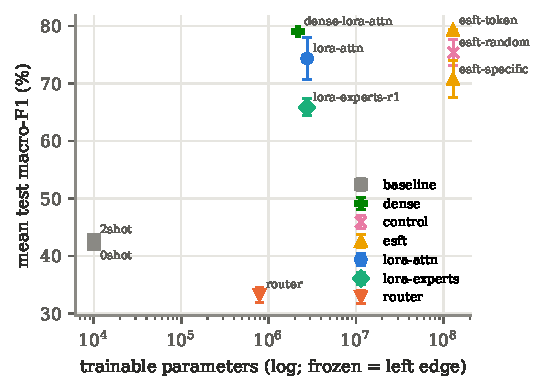
\includegraphics[width=\columnwidth]{figures/pareto}
\caption{Mean test macro-F1 against the number of trainable parameters (mean $\pm$ std over
three seeds; frozen baselines are drawn at the left edge).}
\label{fig:pareto}
\end{figure}

\subsection{Which experts to tune}
The three ESFT variants train the same number of experts in every layer and therefore exactly
the same number of parameters. The choice still matters: ESFT-Token (79.3\%) is ahead of
random experts (75.4\%), which are ahead of our domain-specific selection (70.8\%). The
difference between the variants is again largest on Headlines.

To explain the order, Table~\ref{tab:coverage} measures, for each selection, the share of all
routing decisions on the financial training data that go to the selected experts. Usage-based
selection covers 22.8\% of the routed tokens with 10.7\% of the experts. Random experts cover
roughly their share (10.7\%). The domain-specific experts are the most selective: they are
chosen 1.9 times more often on financial than on general text (9.3\% vs.\ 5.0\%), but they
see fewer financial tokens than random ones. The ranking of macro-F1 follows the coverage
exactly. A tuned expert can only change the output for the tokens routed to it, so the
amount of computation that passes through the adapted parameters, rather than their
specialisation, determines how much the model can change.

\begin{table}[t]
\centering
\caption{Share of routing decisions (top-$k$ slots, averaged over layers) that go to the
experts selected by each ESFT variant, on financial training data and on SST-2. All variants
select 82 of 768 experts (10.7\%).}
\label{tab:coverage}
\begin{tabular}{l c c c}
\toprule
Selection & Financial & General & Mean F1 \\
\midrule
ESFT-Token & 22.8 & 21.0 & 79.3 \\
ESFT-Random & 10.7 & 10.5 & 75.4 \\
ESFT-Specific & 9.3 & 5.0 & 70.8 \\
\bottomrule
\end{tabular}
\end{table}

\subsection{Routing analysis}
\label{sec:routing}

\begin{figure*}[t]
\centering
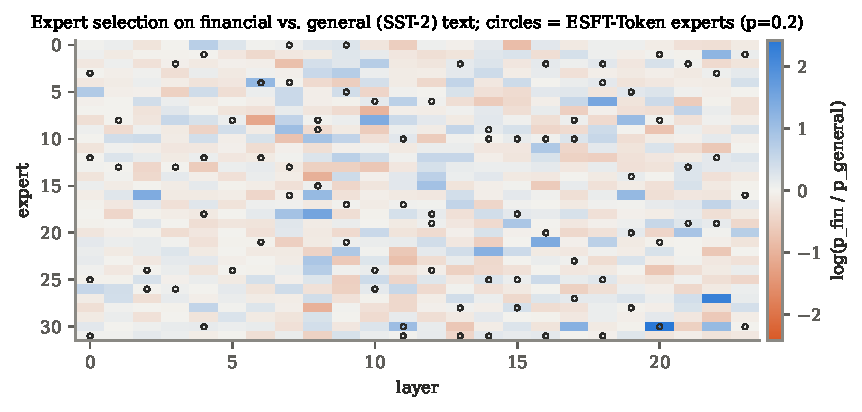
\includegraphics[width=0.85\textwidth]{figures/domain_specificity}
\caption{Domain specificity $\sigma_{\ell,e}$ of every expert of the frozen model (blue: used
more on financial text, orange: more on SST-2). Circles mark the experts selected by
ESFT-Token; most of them lie on neutral cells.}
\label{fig:spec}
\end{figure*}

\textbf{Financial text is routed differently, but only slightly.} Fig.~\ref{fig:sim} shows the
Jensen--Shannon divergence between the per-layer expert distributions of the frozen model on
the financial training sets (up to 1000 examples each) and on SST-2. The three sentiment datasets are close to each other
($2$--$5\cdot10^{-3}$) and farther from SST-2 ($12$--$16\cdot10^{-3}$); Headlines, whose prompts
contain a question, is about as far from the sentiment tasks as SST-2 is. The router entropy is high on every dataset
(3.02--3.06 nats out of a maximum of $\ln 32=3.47$), i.e.\ the model spreads tokens over many
experts and no small group of experts is reserved for finance.

\textbf{High-usage experts are generic.} Fig.~\ref{fig:spec} shows $\sigma_{\ell,e}$ for all
experts. Specificity is concentrated in a few experts per layer, and the experts that ESFT
selects are rarely among them: they are used heavily on financial and on general text alike
(Table~\ref{tab:coverage}). ESFT therefore works not because it finds ``financial experts'',
but because it adapts the experts that handle the largest part of the computation.

\textbf{Router tuning moves the routing far more than the domain does.} Fig.~\ref{fig:shift}
compares the routing of every fine-tuned model with the frozen one on the same test inputs.
Methods that leave the router frozen change it only through the hidden states
(JS $\le 4\cdot10^{-3}$ averaged over layers). The trained router moves it by
$0.14$--$0.16$, about ten times the difference between financial and general text, and the
shift grows with depth. Sending tokens to experts that were not trained to process them
destroys more than the re-routing gains, which explains why this method is below zero-shot.

\begin{figure}[t]
\centering
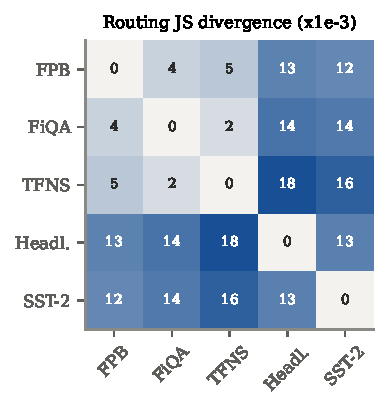
\includegraphics[width=0.78\columnwidth]{figures/task_similarity}
\caption{Routing Jensen--Shannon divergence between datasets (frozen model, financial training
data and SST-2,
averaged over layers).}
\label{fig:sim}
\end{figure}

\begin{figure}[t]
\centering
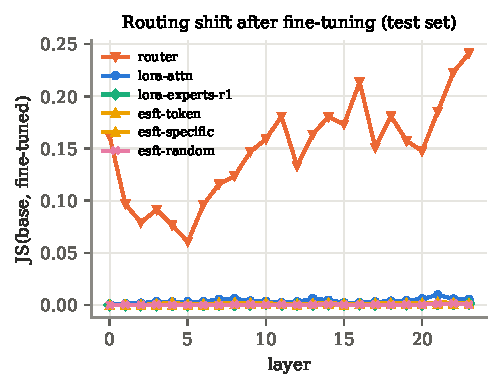
\includegraphics[width=\columnwidth]{figures/routing_shift}
\caption{Per-layer JS divergence between the routing of the frozen model and of each
fine-tuned model (seed 0) on the test sets.}
\label{fig:shift}
\end{figure}

\subsection{Error analysis}
\label{sec:errors}
Table~\ref{tab:recall} reports the recall of the classes that separate the methods, computed
from the saved test predictions and averaged over seeds.

\textbf{The frozen model ignores the neutral class.} Zero-shot, the model labels 0.1\% of the
\fpb{} sentences as neutral, although neutral is the majority class (60\% of the data); neutral
recall is 0.2\% on \fpb{} and 3.2\% on \tfns{}. This is the domain gap from the introduction in
its simplest form: factual statements such as dates, volumes and announcements are read as
positive or negative. Every method that adapts the network body raises neutral recall on
\fpb{} and \tfns{} to 86--92\%, which accounts for most of the improvement on these two tasks.
The router is the exception: it over-corrects and labels 86\% of the \fpb{} sentences as neutral.

\textbf{\fiqa{} is limited by its neutral class.} Only 8\% of the \fiqa{} training posts (about
60 examples) are neutral, and no method except the router, which over-predicts neutral
everywhere, recovers this class: neutral recall stays between 4\% and 22\%. Since macro-F1
weights the three classes equally, this caps \fiqa{} near 60--66\% for all methods, and the
ranking on this task largely follows the neutral recall (ESFT-Token is the best with 22\%).

\textbf{Headlines separates the methods through the minority class.} ``Yes'' answers are 32\%
of the Headlines data. Methods that fail on Headlines mostly stop predicting them: expert LoRA
recalls 2.5\% of them and predicts ``Yes'' for fewer than 1\% of the questions, ESFT-Specific
recalls 22\%. ESFT-Token reaches 64\% and the dense model 77\%, which explains the dense
model's lead on this task. The seed variance of attention LoRA and ESFT-Specific also comes from
this class, and it is already visible on the validation set (for attention LoRA, Headlines
validation macro-F1 is 75.7, 71.4 and 44.8 for the three seeds against 78.7, 70.2 and 51.1 on
test), so it is caused by training rather than by checkpoint selection. Questions about
headlines require relating a templated question to a short text, a different skill from
sentiment; a model that adapts few parameters, or the wrong ones, learns the majority answer.

\begin{table}[t]
\centering
\caption{Test recall (\%) of the neutral class and of ``Yes'' on Headlines, mean over seeds.}
\label{tab:recall}
\begin{tabular}{l c c c c}
\toprule
Method & \fpb{} neu. & \tfns{} neu. & \fiqa{} neu. & Headl. Yes \\
\midrule
Zero-shot & 0.2 & 3.2 & 5.6 & 10.1 \\
Router only & 85.7 & 61.6 & 57.4 & 20.8 \\
LoRA-Experts & 88.7 & 87.0 & 3.7 & 2.5 \\
ESFT-Specific & 88.9 & 89.9 & 5.6 & 21.7 \\
LoRA-Attn & 85.9 & 87.5 & 18.5 & 43.7 \\
ESFT-Random & 88.7 & 90.2 & 7.4 & 50.4 \\
ESFT-Token & 88.7 & 91.5 & 22.2 & 64.3 \\
Dense LoRA-Attn & 88.3 & 91.4 & 11.1 & 77.3 \\
\bottomrule
\end{tabular}
\end{table}

\subsection{Efficiency}
Table~\ref{tab:eff} reports the cost of one run on a T4. ESFT trains 47 times more parameters
than attention LoRA, but the stored adapter is still only 9.7\% of the model, training takes
7 minutes, and the peak memory (12.0\,GB) is 1.7\,GB above LoRA, mostly for the Adam state of
the selected experts. Expert LoRA is the most expensive method in time and memory although it
has few parameters, because every expert is touched and the adapters are applied in a Python
loop over experts. The dense model is about twice as fast and needs half the memory: at this
scale the MoE model has no efficiency advantage in our implementation.

\begin{table}[t]
\centering
\caption{Cost per run on one T4 (mean over seeds): trainable parameters, training time,
peak memory and test latency per example (batch 16).}
\label{tab:eff}
\begin{tabular}{l r r r r}
\toprule
Method & Params & Min & GB & ms \\
\midrule
Router only & 0.79M & 4.7 & 9.3 & 8.9 \\
LoRA-Attn & 2.75M & 5.0 & 10.2 & 9.5 \\
LoRA-Experts & 2.75M & 14.6 & 13.4 & 25.6 \\
ESFT (any) & 129.0M & 6.2--6.9 & 11.5--12.0 & 12.4--13.3 \\
Dense LoRA-Attn & 2.16M & 2.5 & 5.5 & 5.2 \\
\bottomrule
\end{tabular}
\end{table}

\begin{figure}[t]
\centering
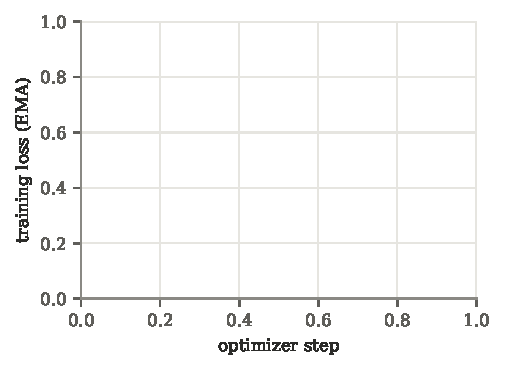
\includegraphics[width=\columnwidth]{figures/training_curves}
\caption{Training loss (exponential moving average, seed 0).}
\label{fig:curves}
\end{figure}

\section{Discussion}

\textbf{Where to spend the parameters.} In this MoE model, the most effective place for
trainable parameters is the experts that already process most of the tokens, updated at full
rank. A small number of parameters works well in the attention, where every token passes,
but the same number spread thinly over all experts does not. Both observations point the
same way: what limits an adapter in a sparse model is how much of the computation it reaches.
Usage-based selection exploits this directly, which is why the original ESFT score works and
our specificity score does not. The result that the most used experts are not
domain-specific agrees with the high router entropy we measure: in a fine-grained model with
top-8 routing, domain knowledge is spread over many shared experts rather than isolated in a
few.

\textbf{Negative result for ESFT-Specific.} Ranking experts by $\log(p_\text{fin}/p_\text{gen})$
finds experts that are indeed more typical of finance, but they are rarely chosen, so their
updates affect few tokens. A score that combines both factors, e.g.\ usage weighted by
specificity, or the same selection with a larger budget, may work better; we did not test it.
Specificity might still be useful when catastrophic forgetting of the general domain matters,
because the selected experts carry only 5\% of the general-domain routing (vs.\ 21\% for ESFT),
but we did not measure forgetting.

\textbf{MoE vs.\ dense.} At the scale we can afford, the MoE model is not better than a dense
model with a similar number of active parameters: ESFT matches the dense model in mean
macro-F1 and accuracy but needs 60 times more trainable parameters, twice the memory and more than
twice the latency. The dense model is clearly better on Headlines, the MoE model on \fiqa{}. The
efficiency gap is partly due to our expert implementation (a loop instead of a fused grouped
GEMM) and would be smaller with optimised kernels.

\textbf{Limitations.}
\begin{itemize}
  \item One MoE model (1.3B) and one dense model; results for large MoE models with fewer,
  bigger experts may differ.
  \item No hyper-parameter search; learning rates follow common practice per method. The
  router may need a much lower learning rate or a regulariser to keep the routing close to
  the pre-trained one, and its failure here is a result for this setting only.
  \item The ESFT variants have about 47 times more trainable parameters than the LoRA methods,
  so the comparison between parameter \emph{locations} is budget-matched only for attention
  vs.\ expert LoRA.
  \item Three seeds; differences below about one standard deviation (e.g.\ ESFT vs.\ the dense
  model) are not significant. Headlines is the most seed-sensitive task, and the mean F1 of
  several methods is dominated by it.
  \item Short single-epoch training on 8.9K examples; we do not evaluate forgetting on general
  data or other financial tasks such as named-entity recognition or question answering.
\end{itemize}

\section{Conclusion}
We compared where to place trainable parameters when adapting a sparse MoE language model to
financial text classification. Updating the experts that the model already uses most (ESFT)
gives the best and the most stable result, comparable to LoRA on a dense model of similar
active size; attention LoRA is a strong cheap alternative, expert LoRA at the same budget is
weaker, and tuning only the router is harmful. Selecting domain-specific instead of frequently
used experts performs worse than random selection, and a routing analysis shows the reason:
the benefit of a tuned expert is proportional to the share of tokens routed to it. For
practitioners, this suggests choosing adapted experts by the amount of computation they
handle on the target data, not by how specialised they look.


\bibliographystyle{IEEEtran}
\bibliography{references}

\end{document}
